\section{Mesh Partitioning}
\label{sec:partitioning}

The hardest task that needs to be done in order to allow a distributed memory implementation of the application is the partitioning of the data. The input consists solely of a two dimensional mesh, constituted by interconnected edges and cells. In each step, every edge and cell needs to access its neighbor cells or edges, respectively.

In order to distribute processing payload across each process, the input mesh, and all of the data associated with it, also needs to be distributed. A mesh partitioning algorithm is required. This algorithm must generate $P$ different partitions (where $P$ is the number of processors), each one corresponding to a subset of the original mesh. Each partition is then assigned to a single processor. Some additional data is also required for each partition so that each process knows how it should communicate with the other partitions, so that the behavior can be simulated as if the mesh is being processed as a whole.

\subsection{Research in Mesh Partitioning}
\label{subsec:part_research}

Mesh partitioning is currently an actively researched topic, and some projects and libraries already exist that help with the understanding of how a mesh (or more generically, a graph) can be partitioned in ways to optimize certain aspects like load balancing, communication balancing or partitioning overhead. For instance, in \cite{metis}, a library called \texttt{Metis} is presented whose purpose is to solve this (and other) problems, by partitioning the mesh into $p$ partitions, roughly equal in size, such that the number of edges connecting multiple partitions is minimized. Other works found for this topic included \cite{gilbert1995,walshaw2000}.

However, given the time constraints of this project, and since the priority was to have a functional algorithm, it was decided not to attempt a mesh partitioning approach that would involve \textit{Metis} or any other researched work. Actually, the method used to partition the mesh is quite naive, as shown in \cref{subsec:part_method}

\subsection{Partitioning Methodology}
\label{subsec:part_method}

The algorithm created to partition the mesh works by dividing the input based on the centroid (the $(x, y)$ coordinates for the center point)) of each cell. Given a mesh with a total of 100 cells, and a pool of $P$ processes, it divides the mesh into $P$ partitions, each one with exactly $N=100/P$ cells, differing by at most one cell if they can't be divided evenly. To select which cells go to which process, the choice is based on the $x$ coordinate of each cell. They are first ordered into a set using $x$ as the ordering key, and then sequentially assigned to each process, in such a way that the first process receives the first $N$ cells of the set, the second process receives the next subset of size $N$, and so on until no more cells are left.

\begin{figure}[!htp]
	\begin{center}
		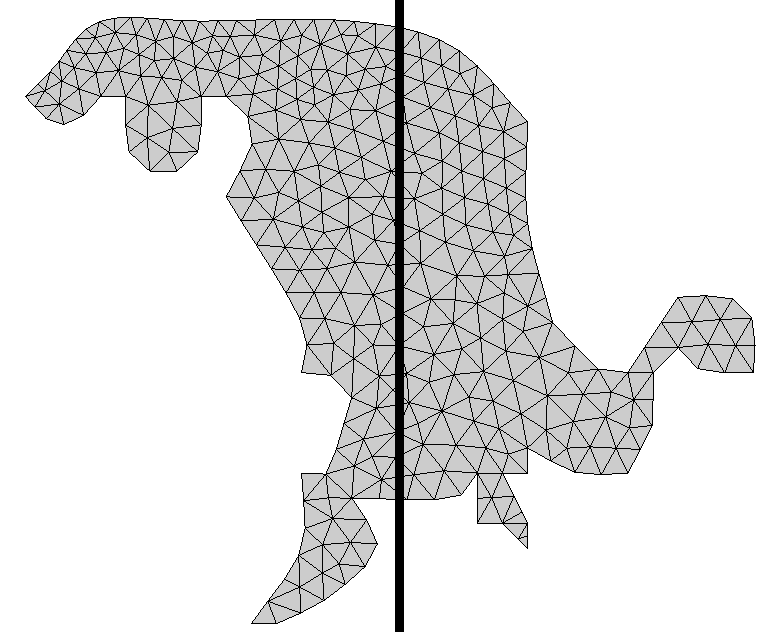
\includegraphics[width=\columnwidth]{report.may/images/foz_p2_msh}
	\end{center}
	\caption{Example of how the mesh will be partitioned when running the algorithm with 2 processes}
	\label{fig:tasktimeAOS}
\end{figure}

\begin{figure}[!htp]
	\begin{center}
		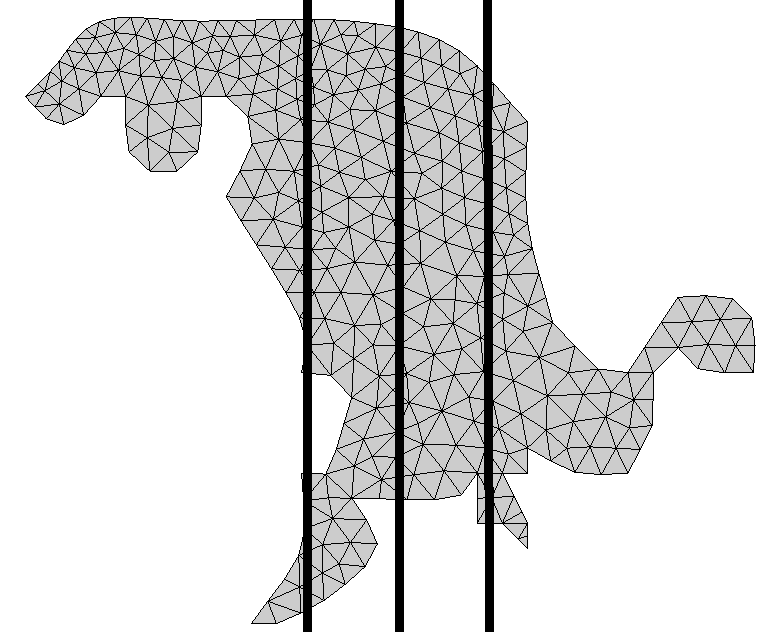
\includegraphics[width=\columnwidth]{report.may/images/foz_p4_msh}
	\end{center}
	\caption{Same example, but with 4 processes. Notice how the width of each partition is different, due the higher concentration of cells in the central area}
	\label{fig:tasktimeAOS}
\end{figure}

This sequential distribution, along with the need to sequentially order every cell of the mesh in order to distribute them, creates a rather large overhead in pre-computational time.

After each cell is assigned, every partition then receives all the edges that are attached to their cells. At this point, some redundancy is created, as edges in the border of one partition will also exist in the neighbor partition.

Some preprocessing is also done at this stage, to index, for each partition, the subset of edges that connect to the left and right neighbors. Since the division is done vertically, by the $x$ coordinate of each cell, it is guaranteed that every partition will have at most two neighbors, one at the left side, and one at the right side (the only exception are the first and last partition which will only have one neighbor). It is also assumed that the width of the global mesh is big enough so that there are never any jumps between partitions, with a partition sharing an edge with another one which is not a direct neighbor of it.

This partitioning method, while guaranteeing that the load balancing is good in terms of amount of work per process, also suffers from not considering the size of the frontier of each partition, which will directly affect the size and overhead of the communication required between partitions.
